\chapter{周期性}\label{ch:b1:periodicity}

锂、钠和钾是柔软、有光泽的金属，在空气中会失去光泽，
并与水反应；氟、氯和溴则是有颜色、有腐蚀性的非金属，
几乎能从任何物质中夺取电子。每组三元素位于元素\omterm{def:b1:periodicity:table}{周期}表的同一列中，
同列元素彼此相似，而同一行中相邻的元素则不然。
上一章已经解释了其中的原因：
同一列的元素具有相同的价电子构型。
本章将这一解释数量化，
引入原子半径、电离能、\omterm{def:b1:periodicity:electron-affinity}{电子亲和能}、\omterm{def:b1:periodicity:electronegativity}{电负性}等物理量——
并归纳出各种变化趋势。借助这些趋势，化学家
仅凭元素在\omterm{def:b1:periodicity:table}{周期}表中的位置，就能预测其原子有多大、
原子多容易失去或获得电子，
以及键合电子偏向哪一方。

\begin{recall}
每一\omterm{def:b1:periodicity:table}{周期}都从 $n$s \omterm{def:b1:quantum-numbers:orbital}{电子亚层}的填充开始，
并以 $n$p \omterm{def:b1:quantum-numbers:orbital}{电子亚层}填满结束；s、p、d 和 f 区的宽度分别为 2、6、10
和 14（见\cref{prop:b1:quantum-numbers:table}）。第 1 册（十一年级）
已经将\omterm{def:b1:periodicity:electronegativity}{电负性}描述为
原子吸引成键电子的倾向。
\end{recall}

\section{由电子构型建立的周期表}

\begin{definition}[周期、族、区]\label{def:b1:periodicity:table}
在元素周期表中，元素按原子序数 $Z$ 递增排列。
\emph{周期}\index{周期}是一行，同一行元素的价\omterm{def:b1:quantum-numbers:orbital}{电子层}具有相同的
\omterm{def:b1:quantum-numbers:quantum-number}{主量子数} $n$。\emph{族}\index{族}是一列，编号为 1 至 18，
同一列元素的价电子构型相同。
\emph{区}\index{区}是末一个填充的\omterm{def:b1:quantum-numbers:orbital}{电子亚层}属于同一类
（s、p、d 或 f）的元素构成的集合。
\end{definition}

\begin{example}[判断元素的位置]\label{ex:b1:periodicity:position}
硒的电子构型为 $[\ce{Ar}]\,3\text{d}^{10} 4\text{s}^2 4\text{p}^4$，
位于第 4 \omterm{def:b1:periodicity:table}{周期}（价\omterm{def:b1:quantum-numbers:orbital}{电子层} $n = 4$），属于 p 区，
位于第 16 族（$2 + 10 + 4$：2 个 s 电子、10 个 d 电子和 4 个 p 电子）；
其价电子构型 $n\text{s}^2 n\text{p}^4$ 与其上方的氧和硫相同。
\end{example}

\begin{definition}[金属、非金属、类金属]\label{def:b1:periodicity:metalloid}
金属是这样一种元素：其固体导电，其原子易失去电子形成阳离子；
非金属是不导电（石墨等少数例外）的元素，
且易获得电子或与其他原子共用电子。
\emph{类金属}\index{类金属}是性质介于两者之间的元素，
属于半导体，
包括硼、硅、锗、砷、锑和碲。
\end{definition}

\begin{omfigure}
\omperiodictable[colour=metals, legend, f block=false]

{\small 金属（占绝大多数）、沿硼至碲阶梯线分布的\omterm{def:b1:periodicity:metalloid}{类金属}，
以及位于右上方的非金属。
此处省略的 f 区由金属构成。}
\end{omfigure}

\section{大小：原子半径与离子半径}

\begin{definition}[屏蔽、有效核电荷]\label{def:b1:periodicity:screening}
在多电子原子中，一个电子受到电荷为 $Ze$ 的原子核吸引，
同时受到其他电子的排斥。\omterm{def:b1:quantum-numbers:configuration}{内层电子}会部分抵消
原子核的吸引，这称为\emph{屏蔽}\index{屏蔽}。\omterm{def:b1:quantum-numbers:configuration}{价电子}
所感受到的核电荷为 $Z^{*}e$，称为\emph{有效核电荷}\index{有效核电荷}，
且 $Z^{*} < Z$。
\omterm{def:b1:quantum-numbers:configuration}{内层电子}几乎完全起屏蔽作用；
同一\omterm{def:b1:quantum-numbers:orbital}{电子层}中的电子
只起很小的屏蔽作用。
\end{definition}

\begin{remark}[定性工具]\label{rem:b1:periodicity:slater}
本书中 $Z^{*}$ 仅作定性使用：沿\omterm{def:b1:periodicity:table}{周期}方向，$Z$ 每步增加 1，
而新加入的电子位于同一\omterm{def:b1:quantum-numbers:orbital}{电子层}，\omterm{def:b1:periodicity:screening}{屏蔽}作用很小，
因此\omterm{def:b1:quantum-numbers:configuration}{价电子}感受到的 $Z^{*}$ 增大；沿族向下，$Z^{*}$ 变化不大，
但价\omterm{def:b1:quantum-numbers:orbital}{电子层} $n$ 增大。
由电子构型计算 $Z^{*}$ 的规则（斯莱特规则）
见本科二年级分册。
\end{remark}

\begin{definition}[共价半径、离子半径]\label{def:b1:periodicity:radius}
元素的\emph{共价半径}\index{共价半径}等于该元素两个原子之间
单键长度的一半：以氯为例，
即 \ce{Cl-Cl} 距离（\ce{Cl2} 分子）的一半。
离子的\emph{离子半径}\index{离子半径}是离子晶体中相邻阳离子与
阴离子之间距离中归属于该离子的部分，
这一归属依据某一约定确定，该约定规定参考离子
（\ce{O^{2-}}）的半径；离子半径与近邻数目略有关。
\end{definition}

\begin{example}[卤素]\label{ex:b1:periodicity:halogen-radii}
\ce{F2}、\ce{Cl2}、\ce{Br2} 和 \ce{I2} 的键长分别为 141.2、
198.8、228.1 和 \qty{266.6}{pm}，因此\omterm{def:b1:periodicity:radius}{共价半径}分别为 71、99、114
和 \qty{133}{pm}：沿族向下每增加一个\omterm{def:b1:quantum-numbers:orbital}{电子层}，半径约增加
\qty{20}{pm} 或更多。
% ledger: re:F2, re:Cl2, re:Br2, re:I2
\end{example}

\begin{proposition}[半径的变化趋势]\label{prop:b1:periodicity:radius-trend}
沿\omterm{def:b1:periodicity:table}{周期}自左向右，原子半径减小；沿族自上而下，
原子半径增大。阳离子比其原子小，阴离子比其原子大；
在等电子系列（即具有相同电子构型的离子）中，
半径随 $Z$ 增大而减小。
\end{proposition}

\begin{proof}[推理]
原子的大小取决于其价轨道的大小，
价轨道随 $Z^{*}$ 增大而收缩，随 $n$ 增大而膨胀。沿\omterm{def:b1:periodicity:table}{周期}方向，$n$ 不变，
而 $Z^{*}$ 增大，原子收缩。沿族向下，$n$ 每步增加 1，
其影响超过 $Z^{*}$ 的微小变化。阳离子失去了价\omterm{def:b1:quantum-numbers:orbital}{电子层}，
或失去了一些相互排斥的电子；阴离子则获得了一个
与其他电子相互排斥的电子。在等电子系列中，相同的电子
受到核电荷不断增大的原子核束缚。
\end{proof}

\begin{omfigure}
\begin{tikzpicture}[font=\small, x=1pt, y=1pt]
  % ledger: rion:O2-VI, rion:F-VI, rion:Na+VI, rion:Mg2+VI, rion:Al3+VI
  % radii in pm drawn at 0.30 pt per pm (circles to scale)
  \foreach \x/\r/\lab/\v in {40/140/\ce{O^{2-}}/140, 130/133/\ce{F-}/133,
      210/102/\ce{Na+}/102, 275/72/\ce{Mg^{2+}}/72, 325/53.5/\ce{Al^{3+}}/54} {
    \draw[fill=omDef!20, draw=omDef!70!black] (\x,0) circle ({0.30*\r});
    \node at (\x,0) {\lab};
    \node[below] at (\x,-50) {\v\,pm};
  }
  \node[anchor=west, align=left] at (350,0) {每个都有十个电子，\\$Z = 8 \to 13$};
\end{tikzpicture}

{\small 等电子系列 $1\text{s}^2 2\text{s}^2 2\text{p}^6$，
按比例绘制（\omterm{def:b1:periodicity:radius}{离子半径}取六配位邻居）。同样的十个电子，
随核电荷增大而收缩。}
\end{omfigure}

\section{能量：电离与电子亲和能}

\begin{definition}[电离能]\label{def:b1:periodicity:ionisation-energy}
元素的\emph{第一电离能}\index{第一电离能} $E_{i1}$
是指在气相中使元素的\omterm{def:b1:quantum-numbers:energy-level}{基态}孤立原子
失去一个电子所需的能量：
\[
  \ce{X(g) -> X+(g) + e-}, \qquad E_{i1} = E(\ce{X+}) + E(\ce{e-}) - E(\ce{X}) > 0 .
\]
\emph{逐级电离能}\index{逐级电离能}
$E_{i2}, E_{i3}, \dots$ 分别是从
\ce{X+}、\ce{X^{2+}}\dots\ 中移去第二个、第三个电子\dots\ 所需的能量。
它们以电子伏特每原子或千焦每摩尔给出
（$\qty{1}{eV} \leftrightarrow \qty{96.49}{kJ/mol}$）。
% ledger: const:NA, const:e (1 eV x N_A = 96.485 kJ/mol)
\end{definition}

\begin{omfigure}
\begin{tikzpicture}
\begin{axis}[
  width=0.92\linewidth, height=6.4cm,
  xmin=0, xmax=37, ymin=0, ymax=27,
  axis x line=bottom, axis y line=left,
  xlabel={原子序数 $Z$}, ylabel={$E_{i1}$ (eV)},
  xtick={2,10,18,36}, ytick={0,5,10,15,20,25},
  tick label style={font=\small}, label style={font=\small},
  clip=false]
\addplot[omDef, thick, mark=*, mark size=1.3pt] table[x=Z, y=IE_eV] {figdata/out/bachelor-1-ionisation-energies.dat};
\node[font=\small, anchor=south] at (axis cs:2,24.6) {He};
\node[font=\small, anchor=south] at (axis cs:10,21.6) {Ne};
\node[font=\small, anchor=south] at (axis cs:18,15.8) {Ar};
\node[font=\small, anchor=south] at (axis cs:36,14.0) {Kr};
\node[font=\small, anchor=north] at (axis cs:3,5.2) {Li};
\node[font=\small, anchor=north] at (axis cs:11,4.9) {Na};
\node[font=\small, anchor=north] at (axis cs:19,4.1) {K};
\node[font=\small, anchor=north] at (axis cs:31,5.8) {Ga};
\node[font=\small, anchor=north] at (axis cs:5,7.9) {B};
\node[font=\small, anchor=north] at (axis cs:8,13.2) {O};
\node[font=\small, anchor=north west] at (axis cs:13.1,6.0) {Al};
\node[font=\small, anchor=north] at (axis cs:16,9.9) {S};
\node[font=\small, anchor=south] at (axis cs:26,8.0) {3d 金属};
\end{axis}
\end{tikzpicture}

{\small 前 36 种元素的\omterm{def:b1:periodicity:ionisation-energy}{第一电离能}。极大值出现在稀有气体处，
极小值出现在碱金属处；B、Al、Ga 处的小凹陷，
以及 O、S 处的小凹陷，都是
\cref{prop:b1:periodicity:ie-anomalies}所述亚层效应的结果。}
\end{omfigure}

\begin{proposition}[电离能的变化规律]\label{prop:b1:periodicity:ie-trend}
\omterm{def:b1:periodicity:ionisation-energy}{第一电离能}沿\omterm{def:b1:periodicity:table}{周期}从碱金属到稀有气体增大，
沿族向下减小。\omterm{def:b1:periodicity:ionisation-energy}{逐级
电离能}总是增大，$E_{i1} < E_{i2} < \dots$，并且
当移去的电子属于内层时，跃升一个很大的倍数。
\end{proposition}

\begin{proof}[推理]
电子离核较远、所受 $Z^{*}$ 较小时，移去它较容易：
沿\omterm{def:b1:periodicity:table}{周期} $Z^{*}$ 增大而半径收缩；沿族向下半径增大。
逐级移去的每个电子都取自电荷更高、体积更小的离子，因此代价更大；
价\omterm{def:b1:quantum-numbers:orbital}{电子层}一旦空了，
下一个电子来自 $n$ 更小的\omterm{def:b1:quantum-numbers:orbital}{电子层}，离核近得多，
几乎完全不受\omterm{def:b1:periodicity:screening}{屏蔽}。
\end{proof}

\begin{example}[镁]\label{ex:b1:periodicity:magnesium}
镁的\omterm{def:b1:periodicity:ionisation-energy}{逐级电离能}依次为 7.65、15.04、80.14
和 \qty{109.27}{eV}。比值 $E_{i2}/E_{i1} \approx 2$ 较为适中；
$E_{i3}/E_{i2} \approx 5.3$ 则是一次跳跃：第三个电子来自
2p 内层。镁失去两个 3s 电子后，停止于
\ce{Mg^{2+}}，具有氖的稀有气体构型。
% ledger: ie:Mg, ie2:Mg, ie3:Mg, ie4:Mg
\end{example}

\begin{omfigure}
\begin{tikzpicture}
\begin{axis}[
  width=0.55\linewidth, height=5.2cm, ybar, bar width=14pt,
  xmin=0.4, xmax=4.6, ymin=1, ymax=300, ymode=log,
  axis x line=bottom, axis y line=left,
  xlabel={移去的电子}, ylabel={$E_{i}$ (eV)},
  xtick={1,2,3,4}, xticklabels={第一, 第二, 第三, 第四},
  tick label style={font=\small}, label style={font=\small},
  nodes near coords={\pgfmathprintnumber[fixed, fixed zerofill, precision=2]{\pgfplotspointmeta}},
  nodes near coords style={font=\scriptsize},
  point meta=rawy]
\addplot[fill=omDef!40, draw=omDef] table[x=k, y=IE_eV] {figdata/out/bachelor-1-ionisation-energies-mg.dat};
\end{axis}
\end{tikzpicture}

{\small 镁的\omterm{def:b1:periodicity:ionisation-energy}{逐级电离能}（对数坐标轴）。
第三个约为第二个的五倍：3s \omterm{def:b1:quantum-numbers:orbital}{电子层}已空，
内层已被触及。}
\end{omfigure}

\begin{proposition}[同一周期中的两个低谷]\label{prop:b1:periodicity:ie-anomalies}
在第 2 和第 3 \omterm{def:b1:periodicity:table}{周期}中，\omterm{def:b1:periodicity:ionisation-energy}{第一电离能}
从第 2 族到第 13 族略有下降（\ce{Be} 到 \ce{B}，\ce{Mg} 到 \ce{Al}），
从第 15 族到第 16 族亦然（\ce{N} 到 \ce{O}，\ce{P} 到 \ce{S}）。
\end{proposition}

\begin{proof}[推理]
在 \ce{B} 和 \ce{Al} 中，被移去的电子是第一个 p 电子，
能量高于 \ce{Be} 和 \ce{Mg} 的 s 电子。在 \ce{O}
和 \ce{S} 中，被移去的电子是第四个 p 电子，它是第一个
与另一电子共占同一轨道（\omorbs{ud,u,u}），两者间的排斥使其
比 \ce{N} 或 \ce{P} 半充满亚层中的电子更易移去
（\omorbs{u,u,u}）。
% ledger: ie:Be, ie:B, ie:N, ie:O, ie:Mg, ie:Al, ie:P, ie:S
\end{proof}

\begin{definition}[电子亲和能]\label{def:b1:periodicity:electron-affinity}
元素的\emph{电子亲和能}\index{电子亲和能} $E_{ea}$，
即孤立原子在\omterm{def:b1:quantum-numbers:energy-level}{基态}时于气相中
俘获一个电子所释放的能量，
\[
  \ce{X(g) + e- -> X-(g)}, \qquad E_{ea} = E(\ce{X}) + E(\ce{e-}) - E(\ce{X-}) .
\]
当阴离子比原子和自由
电子更稳定时，其值为正。
\end{definition}

\begin{example}[卤素及其近邻元素]\label{ex:b1:periodicity:ea}
\ce{F}、\ce{Cl}、\ce{Br} 和 \ce{I} 的\omterm{def:b1:periodicity:electron-affinity}{电子亲和能}依次为 3.40、
3.61、3.36 和 \qty{3.06}{eV}，为所有元素中最大；\ce{O} 和 \ce{S}
的分别为 1.44 和 \qty{2.02}{eV}，\ce{C} 为 \qty{1.26}{eV}，
\ce{Na} 为 \qty{0.55}{eV}。通过俘获一个电子而补全
亚层的原子（卤素）释放大量能量。氮、铍、
镁及稀有气体不能形成稳定的气态阴离子：多出的
电子要么与半充满 p 亚层中的电子配对，要么进入新的
亚层。氟的亲和能小于氯，因为
所加电子挤入较小的 2p \omterm{def:b1:quantum-numbers:orbital}{电子层}。
% ledger: ea:F, ea:Cl, ea:Br, ea:I, ea:O, ea:S, ea:C, ea:Na
\end{example}

\section{电负性与极化率}

\begin{definition}[电负性]\label{def:b1:periodicity:electronegativity}
元素的\emph{电负性}\index{电负性} $\chi$ 衡量其原子在分子中
吸引所形成化学键中电子的倾向。
目前使用两种标度。
\begin{itemize}
  \item 在\emph{鲍林标度}\index{鲍林标度}中，电负性之差由键能
        $D$ 定义：
        \[
          |\chi_A - \chi_B| = \sqrt{\frac{\Delta E}{\qty{1}{eV}}}, \qquad
          \Delta E = D(\text{A--B}) - \tfrac12\big[D(\text{A--A}) +
          D(\text{B--B})\big],
        \]
        标度以 $\chi(\ce{F}) = 3.98$ 为基准。
  \item 在\emph{马利肯标度}\index{马利肯标度}中，
        $\chi_M = \tfrac12\,(E_{i1} + E_{ea})$，以电子伏特为单位。
\end{itemize}
\end{definition}

\begin{remark}[键能为何多出一项]\label{rem:b1:periodicity:pauling}
若键 A--B 的两个原子对其电子的吸引相同，则该键
能约为 A--A 和 B--B 键能的平均值。当一个
原子的\omterm{def:b1:periodicity:electronegativity}{电负性}更大时，该键获得部分离子
性，即 $\ce{A^{\delta+}-B^{\delta-}}$，其静电吸引
使能量增加：$\Delta E > 0$ 反映电子的不均等共享。马利肯
的定义从原子的角度说的是同一件事：一个能紧紧
束缚自身电子（$E_i$ 大）且易接纳额外电子（$E_{ea}$ 大）
的原子，便会吸引成键电子。
\end{remark}

\begin{omfigure}
% ledger: en:H, en:Li, en:Be, en:B, en:C, en:N, en:O, en:F, en:Na, en:Mg,
% en:Al, en:Si, en:P, en:S, en:Cl, en:K, en:Ca, en:Ga, en:Ge, en:As, en:Se,
% en:Br, en:Rb, en:Sr, en:In, en:Sn, en:Sb, en:Te, en:I, en:Cs, en:Ba
\omperiodictable[upto=56, f block=false, numbers=false, highlight colour=omDef!12,
  highlight={F,O,N,Cl}, values={H/2.20,Li/0.98,Be/1.57,B/2.04,C/2.55,N/3.04,O/3.44,F/3.98,
  Na/0.93,Mg/1.31,Al/1.61,Si/1.90,P/2.19,S/2.58,Cl/3.16,K/0.82,Ca/1.00,Ga/1.81,Ge/2.01,
  As/2.18,Se/2.55,Br/2.96,Rb/0.82,Sr/0.95,In/1.78,Sn/1.96,Sb/2.05,Te/2.10,I/2.66,
  Cs/0.79,Ba/0.89}]

{\small 主族元素的鲍林\omterm{def:b1:periodicity:electronegativity}{电负性}（d 区
留空）。它们自左向右、自下而上递增；
\omterm{def:b1:periodicity:electronegativity}{电负性}最大的四种元素 F、O、Cl 与 N 以阴影标出。}
\end{omfigure}

\begin{proposition}[电负性的变化趋势]\label{prop:b1:periodicity:en-trend}
同一\omterm{def:b1:periodicity:table}{周期}内\omterm{def:b1:periodicity:electronegativity}{电负性}递增，同一族内递减：
氟是\omterm{def:b1:periodicity:electronegativity}{电负性}最大的元素，铯和钫是
最小者。两成键原子间的\omterm{def:b1:periodicity:electronegativity}{电负性}差 $\Delta\chi$ 决定了
该键的性质：$\Delta\chi < 0.4$ 时近似非极性共价键，
$0.4 < \Delta\chi < 1.7$ 为极性共价键，$\Delta\chi > 1.7$ 以离子键为主
——三个区间处于连续谱上，并非截然分明的类别。
\end{proposition}

\begin{example}[三种键]\label{ex:b1:periodicity:bonds}
\ce{C-H}：$\Delta\chi = 2.55 - 2.20 = 0.35$，近似非极性；
\ce{O-H}：$3.44 - 2.20 = 1.24$，为极性键，氧带有部分
负电荷；\ce{Na-Cl}：$3.16 - 0.93 = 2.23$，为离子键。
% ledger: en:C, en:H, en:O, en:Na, en:Cl
\end{example}

\begin{definition}[极化率]\label{def:b1:periodicity:polarisability}
原子、离子或分子的\emph{极化率}\index{极化率}，衡量其电子云
在电场作用下变形的难易程度（电场即
相邻离子或偶极子的场）。一个
可极化的物种在电场中获得一个诱导
偶极矩，与电场强度成正比。
\end{definition}

\begin{proposition}[极化率的变化趋势]\label{prop:b1:periodicity:polarisability-trend}
\omterm{def:b1:periodicity:polarisability}{极化率}随电子云的增大和电子数的增多而增大，
随保持电子的原子核电荷的增大而减小：同一族中自上而下增大
（$\ce{F-} < \ce{Cl-} < \ce{Br-} <
\ce{I-}$）；阴离子的\omterm{def:b1:periodicity:polarisability}{极化率}远大于阳离子，
常见物种中，像 \ce{I-} 这样大而软的阴离子的\omterm{def:b1:periodicity:polarisability}{极化率}最大。
\end{proposition}

\begin{example}[极化率为何重要]\label{ex:b1:periodicity:pol}
分子间的伦敦力，在
\cref{ch:b1:intermolecular-forces-solvents}中讨论，随\omterm{def:b1:periodicity:polarisability}{极化率}增大而增强：
室温下碘单质为固体，氯单质则为气体。在离子
晶体中，小而高电荷的阳离子会使大的阴离子极化，
使键带有一定的共价性，这正是简单离子模型失效之处，已在
\cref{ch:b1:crystals-ionic-covalent}中提及。
\end{example}

\begin{history}[鲍林标度，1932 年]
1932 年，美国化学家莱纳斯·鲍林注意到，两个不同原子之间的
键能几乎总是大于两个对称键键能的平均值，
并由这一超出量建立了第一个\omterm{def:b1:periodicity:electronegativity}{电负性}标度。
随着测得的键能越来越精确，该标度经修订，
至今仍是各种表格中采用的标度。
鲍林于 1954 年获得诺贝尔化学奖，表彰其在
化学键方面的工作，并于 1962 年获得诺贝尔和平奖。
\end{history}

\begin{omfigure}
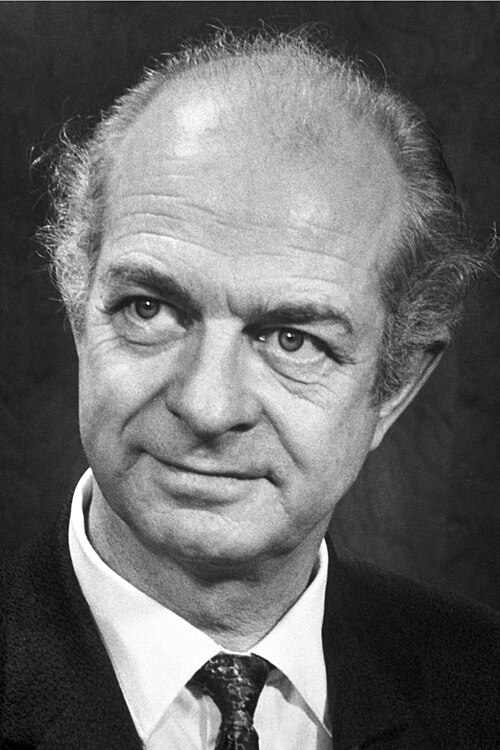
\includegraphics[width=0.24\linewidth]{images/book2/pauling.jpg}

{\small 莱纳斯·鲍林（1901--1994）。}
\end{omfigure}

\section{化学性质的变化趋势}

\begin{proposition}[还原性与氧化性]\label{prop:b1:periodicity:redox-trend}
电离能和\omterm{def:b1:periodicity:electronegativity}{电负性}较低的元素位于\omterm{def:b1:periodicity:table}{周期}表左侧，
以及各自所在族的下部，容易失去电子：
它们是还原性金属（以碱金属最为突出）。\omterm{def:b1:periodicity:electronegativity}{电负性}和\omterm{def:b1:periodicity:electron-affinity}{电子亲和能}较高的元素
位于右上方，容易
得到电子：它们是氧化性非金属（以氟、氧和氯最为突出）。稀有气体电离能高，
且对额外电子没有亲和力，
因此两种性质都不具备。
\end{proposition}

\begin{method}[由位置预测变化趋势]\label{met:b1:periodicity:predict}
比较两种元素在与原子核束缚\omterm{def:b1:quantum-numbers:configuration}{价电子}有关的性质
上的差异（半径、$E_i$、$E_{ea}$、$\chi$）时：
\begin{enumerate}
  \item 若二者位于同一族，位置靠下者的
        $n$ 较大：半径较大，$E_i$ 和 $\chi$ 较小；
  \item 若二者位于同一\omterm{def:b1:periodicity:table}{周期}，位置靠右者的
        $Z^{*}$ 较大：半径较小，$E_i$ 和 $\chi$ 较大；
  \item 其他情况下，将每种元素与其所在行和另一元素所在列交叉处的
        元素进行比较；
  \item 在对电离能下结论之前，检查亚层效应（p 亚层
        的开始、第一个成对的 p 电子）。
\end{enumerate}
\end{method}

\begin{example}[电池中的锂]\label{ex:b1:periodicity:lithium}
锂是第 2 \omterm{def:b1:periodicity:table}{周期}中\omterm{def:b1:periodicity:electronegativity}{电负性}最低的元素，容易失去其 2s
电子，同时它又是最轻的金属：每克所能转移的电荷量
在所有元素中最多，这也正是它能用于
可充电电池的原因。其\omterm{def:b1:periodicity:ionisation-energy}{第一电离能} \qty{5.39}{eV}，
大于钠（5.14）或钾（4.34）的电离能，但在水中它却是
最强的碱金属还原剂，这一矛盾可由小半径 \ce{Li+} 离子的强水合作用来解释
（见\cref{ch:b1:nernst}）。
% ledger: ie:Li, ie:Na, ie:K
\end{example}

\section{练习}

\begin{exercise}[$\star$]\label{exo:b1:periodicity:1}
由\omterm{def:b1:quantum-numbers:configuration}{电子排布}确定钙、铁、硒和
碘（$Z = 20, 26, 34, 53$）的\omterm{def:b1:periodicity:table}{周期}、族和区。
\end{exercise}

\begin{exercise}[$\star$]\label{exo:b1:periodicity:2}
在每一对中，哪一物种更大？为什么？\ce{Na} 或 \ce{Cl}；
\ce{Na} 或 \ce{Na+}；\ce{F-} 或 \ce{Cl-}；\ce{Na+} 或 \ce{Mg^{2+}}。
\end{exercise}

\begin{exercise}[$\star$]\label{exo:b1:periodicity:3}
\ce{Na}、\ce{Mg}、\ce{Al}、\ce{P}、
\ce{S} 和 \ce{Ar} 的\omterm{def:b1:periodicity:ionisation-energy}{第一电离能}分别为 5.14、7.65、5.99、10.49、10.36 和
\qty{15.76}{eV}。将它们排序，并指出两处偏离
一般趋势之处。
\end{exercise}

\begin{exercise}[$\star$]\label{exo:b1:periodicity:4}
给出某物种\omterm{def:b1:periodicity:polarisability}{极化率}的定义。\ce{F-} 与
\ce{I-} 中哪个\omterm{def:b1:periodicity:polarisability}{极化率}更大？\ce{Na+} 与 \ce{Cl-} 中哪个更大？请说明理由。
\end{exercise}

\begin{exercise}[$\star\star$]\label{exo:b1:periodicity:5}
某第 3 \omterm{def:b1:periodicity:table}{周期}元素的前四级电离能分别为 5.99、
18.83、28.45 和 \qty{119.99}{eV}。计算相邻电离能之比，
确定该元素及其形成的离子。
\end{exercise}

\begin{exercise}[$\star\star$]\label{exo:b1:periodicity:6}
解释为什么氯的\omterm{def:b1:periodicity:electron-affinity}{电子亲和能}大于氟，以及为什么
氮和镁不能形成稳定的气态阴离子。
\end{exercise}

\begin{exercise}[$\star\star$]\label{exo:b1:periodicity:7}
计算钠的马利肯\omterm{def:b1:periodicity:electronegativity}{电负性}（$E_{i1} =
\qty{5.14}{eV}$，$E_{ea} = \qty{0.55}{eV}$）以及氯的马利肯\omterm{def:b1:periodicity:electronegativity}{电负性}（$E_{i1} =
\qty{12.97}{eV}$，$E_{ea} = \qty{3.61}{eV}$）。这些结果说明
\ce{NaCl} 中的化学键是什么情况？
\end{exercise}

\begin{exercise}[$\star\star$]\label{exo:b1:periodicity:8}
依据\cref{ex:b1:periodicity:bonds}中的鲍林值，取 $\chi(\ce{F})
= 3.98$，对键 \ce{H-F}、\ce{C-H}、\ce{Na-Cl}、\ce{C-Cl}
（$\chi(\ce{Cl}) = 3.16$）和 \ce{O-H} 进行分类，
并写出每个原子上部分电荷的符号。
\end{exercise}

\begin{exercise}[$\star\star$]\label{exo:b1:periodicity:9}
\ce{Li}、\ce{Na}、\ce{K} 的\omterm{def:b1:periodicity:ionisation-energy}{第一电离能}分别为 5.39、
5.14 和 \qty{4.34}{eV}。解释该变化趋势，并预测铷的
\omterm{def:b1:periodicity:ionisation-energy}{第一电离能}高于还是低于 \qty{4.34}{eV}。
\end{exercise}

\begin{exercise}[$\star\star\star$]\label{exo:b1:periodicity:10}
锌（$Z = 30$）的\omterm{def:b1:periodicity:ionisation-energy}{第一电离能}为 \qty{9.39}{eV}，
镓（$Z = 31$）为 \qty{6.00}{eV}；砷（$Z = 33$）为 \qty{9.79}{eV}，
硒（$Z = 34$）为 \qty{9.75}{eV}。请解释这两处的
下降，借助\omterm{def:b1:quantum-numbers:configuration}{电子排布}加以说明。
\end{exercise}

\begin{exercise}[$\star\star\star$]\label{exo:b1:periodicity:11}
取 $D(\ce{H-H}) = \qty{436}{kJ/mol}$、$D(\ce{F-F}) =
\qty{158}{kJ/mol}$、$\chi(\ce{H}) = 2.20$ 和 $\chi(\ce{F}) = 3.98$，并取
$\qty{1}{eV} = \qty{96.5}{kJ/mol}$。利用鲍林的定义估算
键能 $D(\ce{H-F})$。为何它远大于两个对称键的
键能平均值？
\end{exercise}

\begin{exercise}[$\star\star\star$]\label{exo:b1:periodicity:12}
表中给出了氪（3.00）和氙
（2.60）的鲍林\omterm{def:b1:periodicity:electronegativity}{电负性}，而氦、氖、氩则没有。利用该标度的定义，
解释为何只有能形成键的元素才能给出数值，
以及为何较重的稀有气体恰好能够成键。
% ledger: en:Kr, en:Xe
\end{exercise}

\section{问题：鲍林的计算}

\begin{problem}[{周末问题 --- 由电离能判断一种未知元素，
具有相同大小电子云的一系列离子，两种电负性标度，
以及 H--Cl 键的鲍林数值}]
\label{pb:b1:periodicity:1}
数据：每个粒子 $\qty{1}{eV}$ 相当于 \qty{96.485}{kJ/mol}。

\medskip
\noindent\textbf{第一部分 --- 一种未知元素。}
第 3 \omterm{def:b1:periodicity:table}{周期}元素 X 的前四个电离能依次为 7.65、
15.04、80.14 和 \qty{109.27}{eV}。
\begin{enumerate}
  \item 为什么每一个电离能都大于前一个？
  \item 计算比值 $E_{i2}/E_{i1}$、$E_{i3}/E_{i2}$ 和
        $E_{i4}/E_{i3}$。
  \item 推断 X 所在的族，并确定其元素。
  \item X 在化合物中形成哪种离子？写出其\omterm{def:b1:quantum-numbers:configuration}{电子排布}。
  \item X 是金属还是非金属？请根据其在\omterm{def:b1:periodicity:table}{周期}表中的位置说明理由。
  \item 为什么第三个电子所需的能量远大于第二个？
\end{enumerate}

\medskip
\noindent\textbf{第二部分 --- 十电子体系。}
\omterm{def:b1:periodicity:radius}{离子半径}（六配位）：\ce{O^{2-}}、\ce{F-}、\ce{Na+}、
\ce{Mg^{2+}} 和 \ce{Al^{3+}} 依次为 140、133、102、72 和 \qty{54}{pm}。
\begin{enumerate}[resume]
  \item 证明这些离子具有相同的\omterm{def:b1:quantum-numbers:configuration}{电子排布}。
  \item 解释这些半径的排序。
  \item 五种离子中哪一种的\omterm{def:b1:periodicity:polarisability}{极化率}最大？为什么？
  \item 计算最大半径与最小半径之比。
  \item \ce{Cl2} 的键长为 \qty{198.8}{pm}，
        \ce{Cl-} 的半径为 \qty{181}{pm}。计算氯的\omterm{def:b1:periodicity:radius}{共价半径}，
        并加以比较。
  \item 在没有更多数据的情况下，将 \ce{Cl-}、\ce{Na+} 和 \ce{Mg^{2+}}
        按半径大小排序。
\end{enumerate}

\medskip
\noindent\textbf{第三部分 --- \omterm{def:b1:periodicity:electronegativity}{马利肯标度}。}
\begin{center}
\small
\begin{tabular}{lccccc}
\hline
元素 & \ce{F} & \ce{Cl} & \ce{Br} & \ce{O} & \ce{C} \\
\hline
$E_{i1}$（eV） & 17.42 & 12.97 & 11.81 & 13.62 & 11.26 \\
$E_{ea}$（eV） & 3.40 & 3.61 & 3.36 & 1.44 & 1.26 \\
鲍林 $\chi$ & 3.98 & 3.16 & 2.96 & 3.44 & 2.55 \\
\hline
\end{tabular}
\end{center}
% ledger: ie:F, ie:Cl, ie:Br, ie:O, ie:C, ea:F, ea:Cl, ea:Br, ea:O, ea:C,
% en:F, en:Cl, en:Br, en:O, en:C
\begin{enumerate}[resume]
  \item 计算这五种元素的马利肯\omterm{def:b1:periodicity:electronegativity}{电负性}。
  \item 在两种标度上分别对它们排序，哪一种元素的位置不同？
  \item 计算三种卤素的 $\chi_{\text{鲍林}}/\chi_M$
        比值，你发现了什么？
  \item 请分析为何氧偏离卤素的规律（请看
        其\omterm{def:b1:periodicity:electron-affinity}{电子亲和能}）。
  \item 在 \ce{HCl} 中哪个原子带部分负电荷？在
        \ce{ClF} 中呢？
  \item 取表中数值（$\chi(\ce{H}) = 2.20$），\ce{H-Cl} 键
        是非极性键、极性共价键还是离子键？
\end{enumerate}

\medskip
\noindent\textbf{第四部分 --- H--Cl 键的鲍林数值。}
标准生成焓：\ce{H(g)}、\ce{Cl(g)} 和
\ce{HCl(g)} 在 \qty{298}{K} 下分别为 218.0、121.3 和 \qty{-92.3}{kJ/mol}；
\ce{H2(g)} 和 \ce{Cl2(g)} 的标准生成焓均为零。分子的键能
取为其解离为原子时的焓变。
% ledger: janaf:H, janaf:Cl, janaf:HCl
\begin{enumerate}[resume]
  \item 计算 $D(\ce{H-H})$，所用反应为 \ce{H2(g) -> 2H(g)}。
  \item 计算 $D(\ce{Cl-Cl})$。
  \item 计算 $D(\ce{H-Cl})$，所用反应为 \ce{HCl(g) -> H(g) + Cl(g)}。
  \item 计算鲍林过剩能量 $\Delta E$（以 kJ/mol 为单位），并证明
        它等于 $-\Delta_f H(\ce{HCl})$。
  \item 将 $\Delta E$ 换算为电子伏特。
  \item 计算 $|\chi(\ce{Cl}) - \chi(\ce{H})|$，并将其与
        表中数值之差 $3.16 - 2.20$ 相比较。
\end{enumerate}
\end{problem}
